
The results of the search are shown in
Table~\ref{tab:result}, including both statistical and systematic
uncertainties. Agreement is observed between the data and the
predicted background for all signal regions.  
The predicted and observed \met\ distribution for $\met>150$ GeV and
$\mt>120$ GeV are shown in Figure~\ref{fig:resultsummary}, obtained
from the yields for SRB to SRG. Two signal points are shown for comparison,
corresponding to the low and high stop mass sensitivity
boundaries for this search. This shows that the lower \met\ region is
more sensitive to lighter stop signals, while the higher \met\
region is more sensitive to heavier stops, for the T2tt signal model
shown. The $M_T$ distributions for increasing values of \met\
are shown in Fig~\ref{fig:mtsig1} and \ref{fig:mtsig2}.


	\begin{table}[!h]																															
	\begin{center}																															
	{\footnotesize																															
	\begin{tabular}{l||c|c|c|c|c|c|c}																															
	\hline																															
	Sample		&	SRA			&	SRB			&	SRC			&	SRD			&	SRE			&	SRF			&	SRG\\				
	\hline																															
	\hline																															
	\multicolumn{8}{c}{Muon}	\\																														
	\hline																															
	\ttdl\  		&$	330.6	\pm	21.9	$&$	183.4	\pm	20.7	$&$	59.5	\pm	10.0	$&$	22.5	\pm	6.2	$&$	9.0	\pm	3.9	$&$	3.7	\pm	1.8	$&$	2.2	\pm	1.2	$	\\
	\ttsl\ \& single top (1\Lep) 		&$	92.8	\pm	27.5	$&$	41.0	\pm	8.6	$&$	11.5	\pm	3.5	$&$	7.7	\pm	3.4	$&$	0.7	\pm	0.6	$&$	0.3	\pm	0.2	$&$	0.2	\pm	0.2	$	\\
	\wjets\ 		&$	19.2	\pm	4.5	$&$	10.0	\pm	2.2	$&$	3.1	\pm	1.0	$&$	1.2	\pm	0.6	$&$	0.6	\pm	0.4	$&$	0.4	\pm	0.3	$&$	0.2	\pm	0.2	$	\\
	Rare 		&$	33.2	\pm	16.6	$&$	22.7	\pm	11.4	$&$	9.0	\pm	4.5	$&$	4.8	\pm	2.4	$&$	2.9	\pm	1.5	$&$	1.2	\pm	0.6	$&$	1.0	\pm	0.5	$	\\
	\hline																															
	Total 		&$	475.8	\pm	37.8	$&$	257.2	\pm	24.2	$&$	83.2	\pm	11.3	$&$	36.2	\pm	7.4	$&$	13.3	\pm	4.2	$&$	5.5	\pm	1.9	$&$	3.6	\pm	1.3	$	\\
	\hline																															
	\hline																															
	Data 		&$	?			$&$	?			$&$	?			$&$	?			$&$	?			$&$	?			$&$	?			$	\\
	\hline																															
	\hline																															
	\hline																															
	\multicolumn{8}{c}{Electron}	\\																														
	\hline																															
	\ttdl\  		&$	248.1	\pm	16.9	$&$	144.4	\pm	16.6	$&$	51.1	\pm	8.8	$&$	16.2	\pm	4.6	$&$	5.5	\pm	2.5	$&$	2.5	\pm	1.3	$&$	1.3	\pm	0.7	$	\\
	\ttsl\ \& single top (1\Lep) 		&$	68.0	\pm	20.2	$&$	31.2	\pm	6.6	$&$	9.3	\pm	2.8	$&$	4.9	\pm	2.1	$&$	0.5	\pm	0.4	$&$	0.2	\pm	0.2	$&$	0.2	\pm	0.2	$	\\
	\wjets\ 		&$	14.3	\pm	3.3	$&$	7.5	\pm	1.7	$&$	2.4	\pm	0.8	$&$	0.8	\pm	0.4	$&$	0.4	\pm	0.3	$&$	0.3	\pm	0.2	$&$	0.1	\pm	0.2	$	\\
	Rare 		&$	25.8	\pm	12.9	$&$	15.8	\pm	7.9	$&$	7.1	\pm	3.6	$&$	2.9	\pm	1.5	$&$	0.7	\pm	0.4	$&$	0.3	\pm	0.2	$&$	0.1	\pm	0.1	$	\\
	\hline																															
	Total 		&$	356.2	\pm	28.4	$&$	198.9	\pm	19.0	$&$	69.9	\pm	9.7	$&$	24.7	\pm	5.3	$&$	7.1	\pm	2.5	$&$	3.4	\pm	1.3	$&$	1.7	\pm	0.8	$	\\
	\hline																															
	\hline																															
	Data 		&$	?			$&$	?			$&$	?			$&$	?			$&$	?			$&$	?			$&$	?			$	\\
	\hline																															
	\hline																															
	\hline																															
	\multicolumn{8}{c}{Muon+Electron Combined}		\\																													
	\hline																															
	\ttdl\  		&$	578.7	\pm	38.1	$&$	327.8	\pm	36.6	$&$	110.6	\pm	18.3	$&$	38.7	\pm	10.5	$&$	14.5	\pm	6.2	$&$	6.2	\pm	2.9	$&$	3.5	\pm	1.8	$	\\
	\ttsl\ \& single top (1\Lep) 		&$	160.8	\pm	47.7	$&$	72.2	\pm	15.1	$&$	20.8	\pm	6.3	$&$	12.6	\pm	5.4	$&$	1.2	\pm	0.9	$&$	0.6	\pm	0.4	$&$	0.4	\pm	0.3	$	\\
	\wjets\ 		&$	33.5	\pm	8.0	$&$	17.5	\pm	4.1	$&$	5.5	\pm	1.9	$&$	2.0	\pm	1.2	$&$	1.0	\pm	0.7	$&$	0.7	\pm	0.5	$&$	0.3	\pm	0.4	$	\\
	Rare 		&$	59.0	\pm	29.5	$&$	38.5	\pm	19.3	$&$	16.1	\pm	8.1	$&$	7.7	\pm	3.9	$&$	3.6	\pm	1.8	$&$	1.5	\pm	0.8	$&$	1.1	\pm	0.6	$	\\
	\hline																															
	Total 		&$	832.0	\pm	65.7	$&$	456.1	\pm	42.5	$&$	153.0	\pm	20.6	$&$	60.9	\pm	12.4	$&$	20.3	\pm	6.5	$&$	8.9	\pm	3.0	$&$	5.3	\pm	1.9	$	\\
	\hline																															
	\hline																															
	Data 		&$	?			$&$	?			$&$	?			$&$	?			$&$	?			$&$	?			$&$	?			$	\\
	\hline																															
	\end{tabular}}																															
	\caption{The result of the search.																															
	\label{tab:result}																															
	\end{center}}																															
	\end{table}																															


\begin{table}[!h]
\begin{center}
\begin{tabular}{l|c|c|c|c|c|c|c}
\hline
\hline
                  & SRA & SRB & SRC & SRD & SRE & SRF & SRG \\
\hline
Minimum \mt\  [GeV]  & 150 & 120 & 120 & 120 & 120 & 120 & 120 \\
Minimum \met\  [GeV] & 100 & 150 & 200 & 250 & 300 & 350 & 400 \\
\hline
Total background & $927\pm138$ & $504\pm65$ & $161\pm26$ & $56\pm12$ & $22\pm7$ & $10\pm3.0$ & $5.7\pm2.2$ \\
Data             & 861 & 456 & 150 & 61 & 23 & 9 & 3 \\
\hline
\hline
\end{tabular}
\caption{ Condensed version of the results presented in Table~\ref{tab:result}
\label{tab:result_small}}
\end{center}
\end{table}


\begin{figure}[hbt]
  \begin{center}
        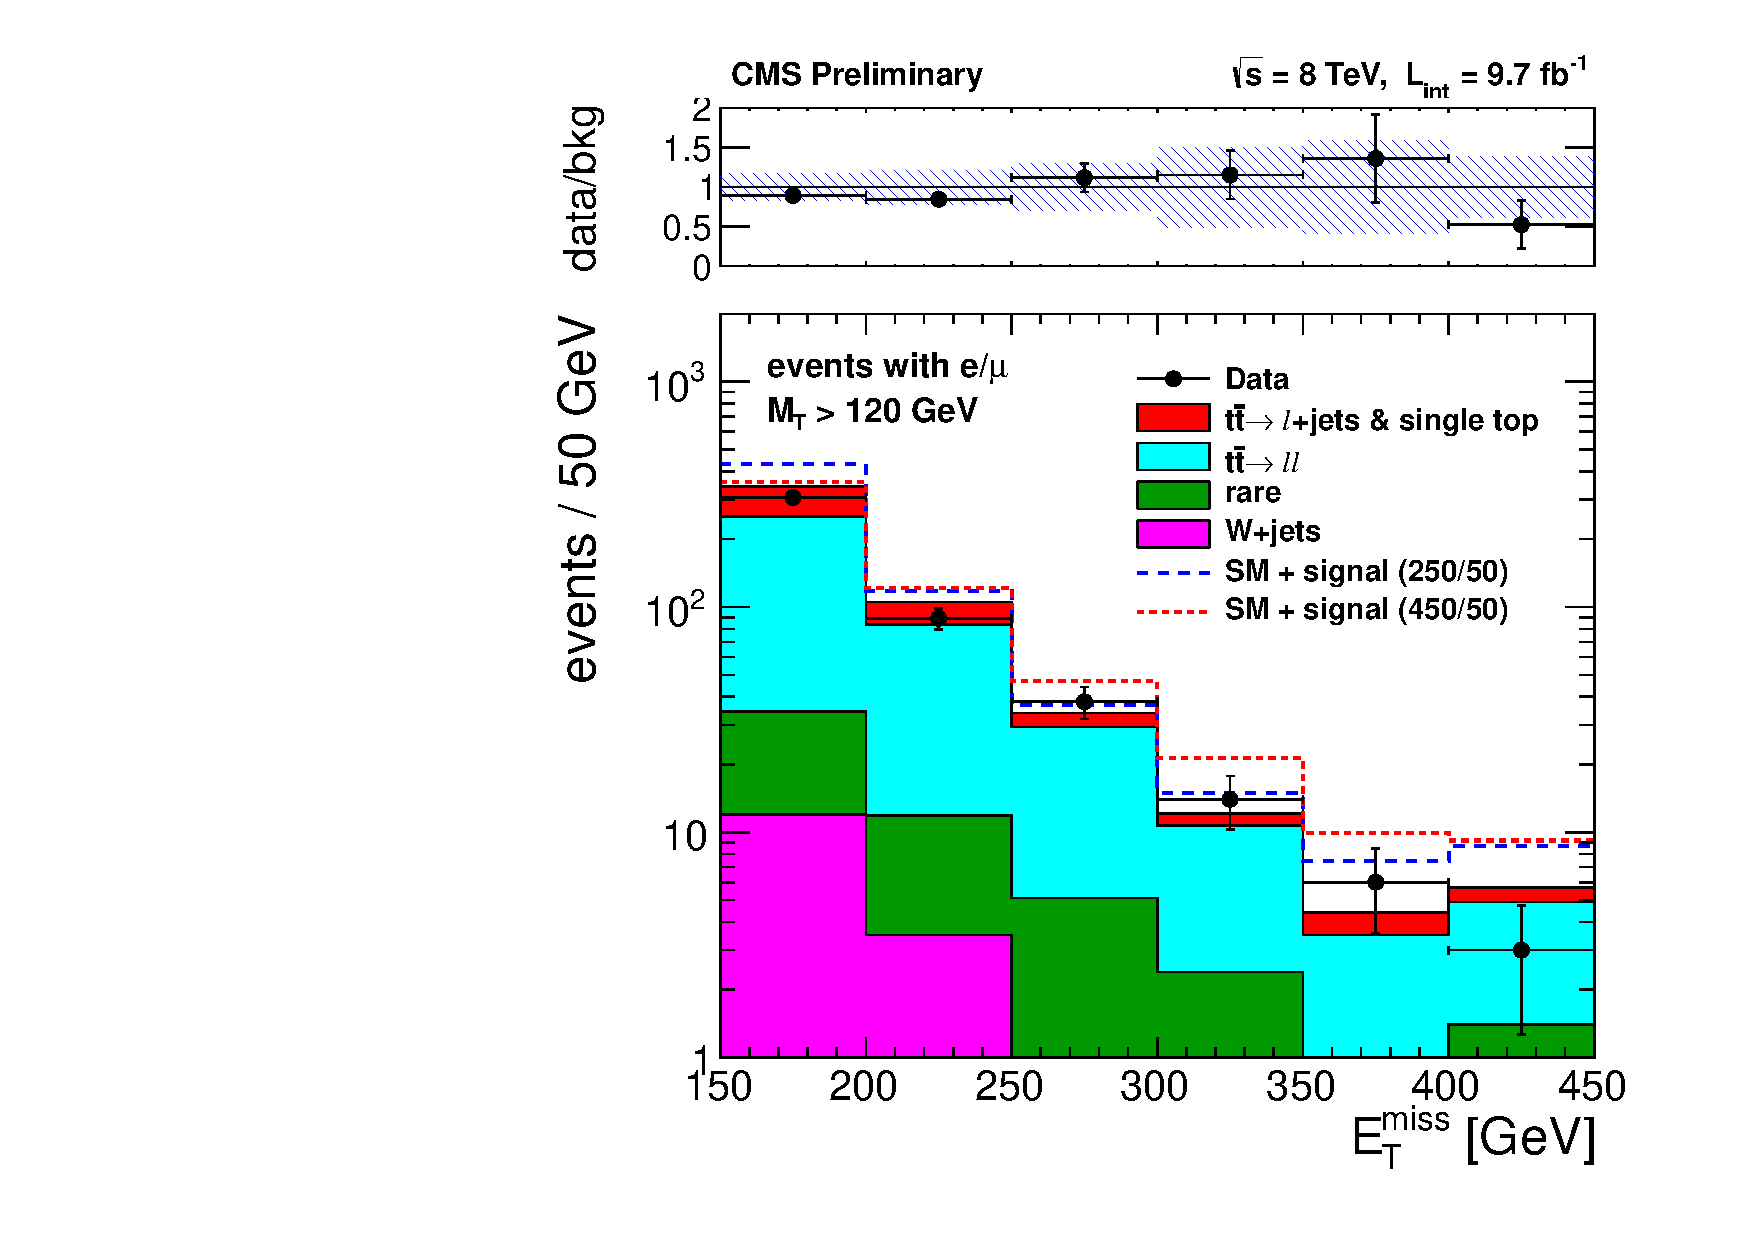
\includegraphics[width=0.75\linewidth]{plots/summaryPlot.pdf}
    \caption{Predicted and observed \met\ for $\mt>120$ GeV, obtained
      from the yields for SRB to SRG. Note SRB corresponds to the integral
      of the distribution, while subsequent signal regions SRC to SRG
      correspond to integrals from subsequent bins. The band on the
      ratio (above) corresponds to the full relative background
      uncertainty. 
\label{fig:resultsummary}
}  
      \end{center}
\end{figure}


\begin{figure}[hbt]
  \begin{center}
        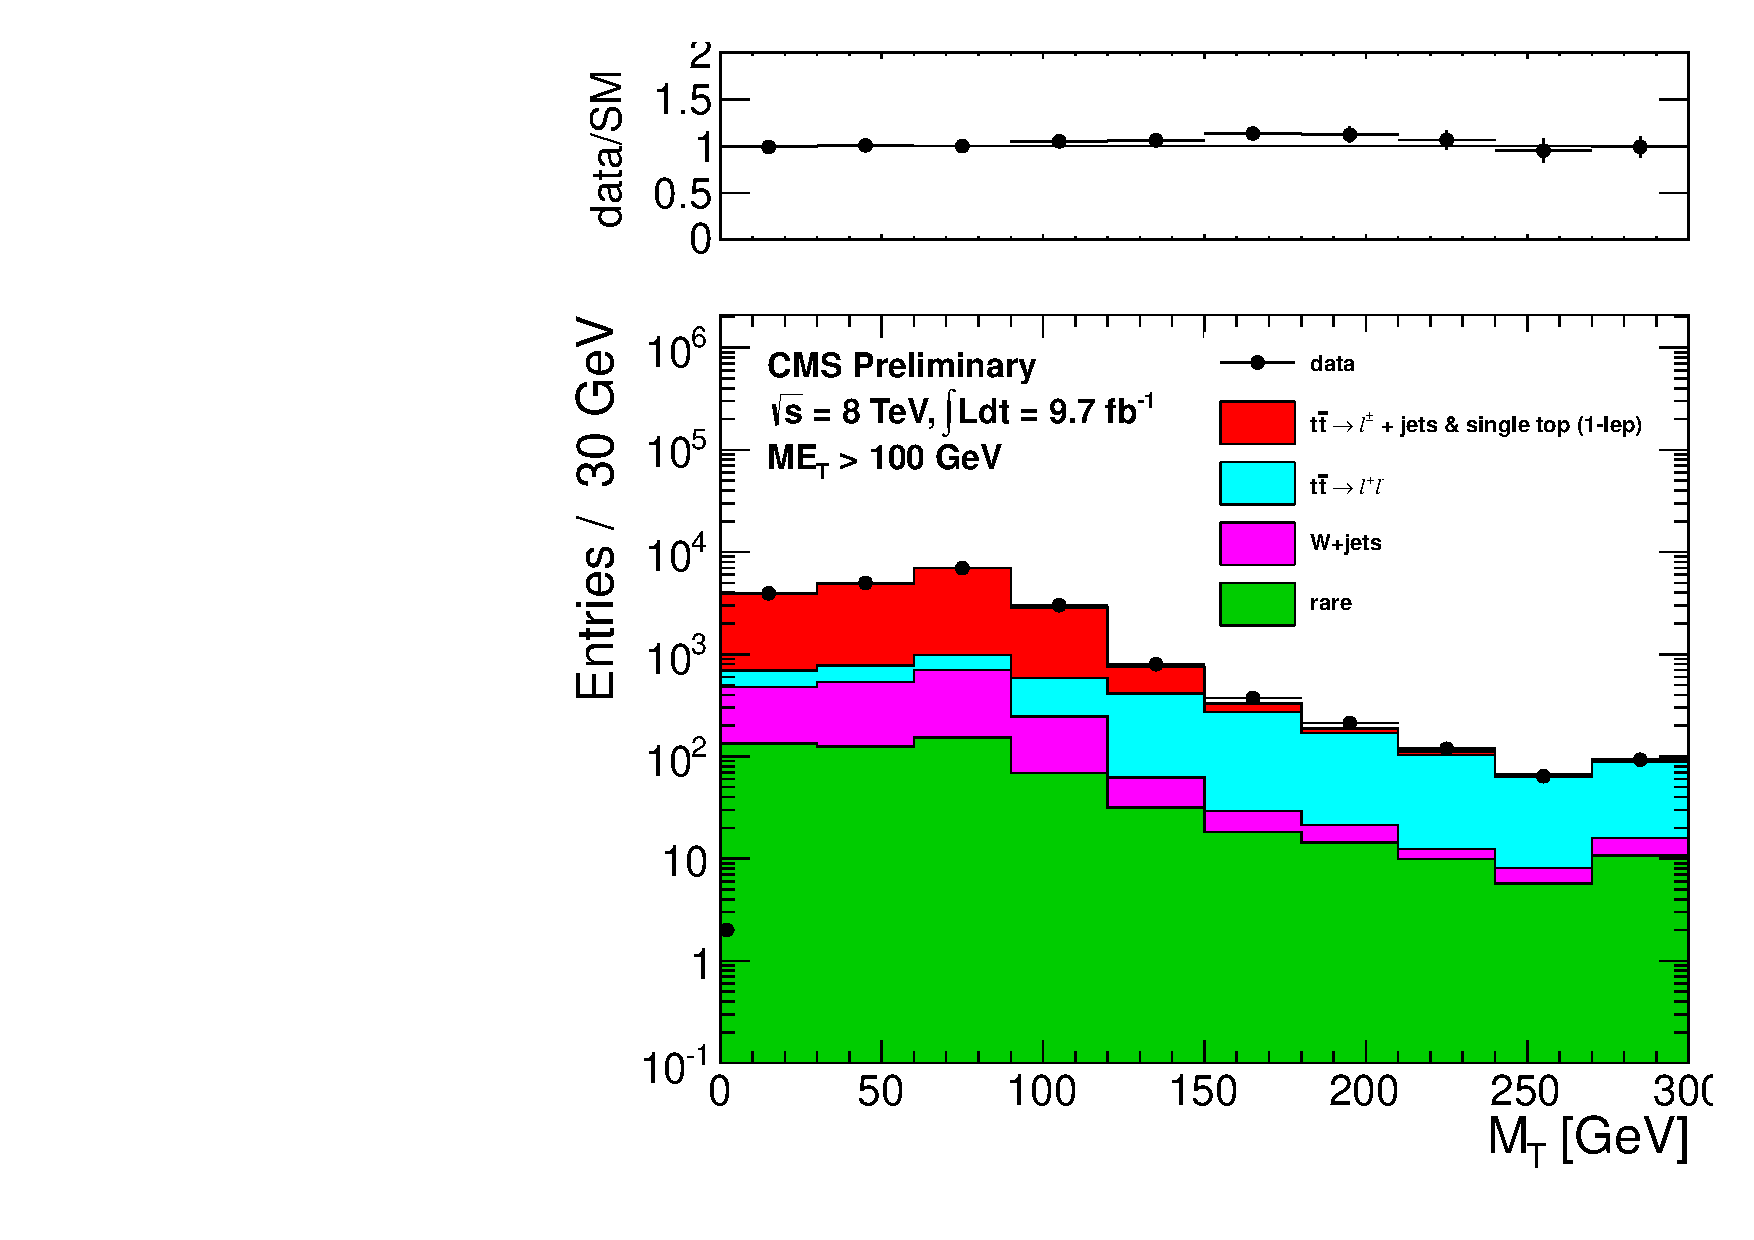
\includegraphics[width=0.5\linewidth]{plots/mt_met100_emucomb.pdf}%
        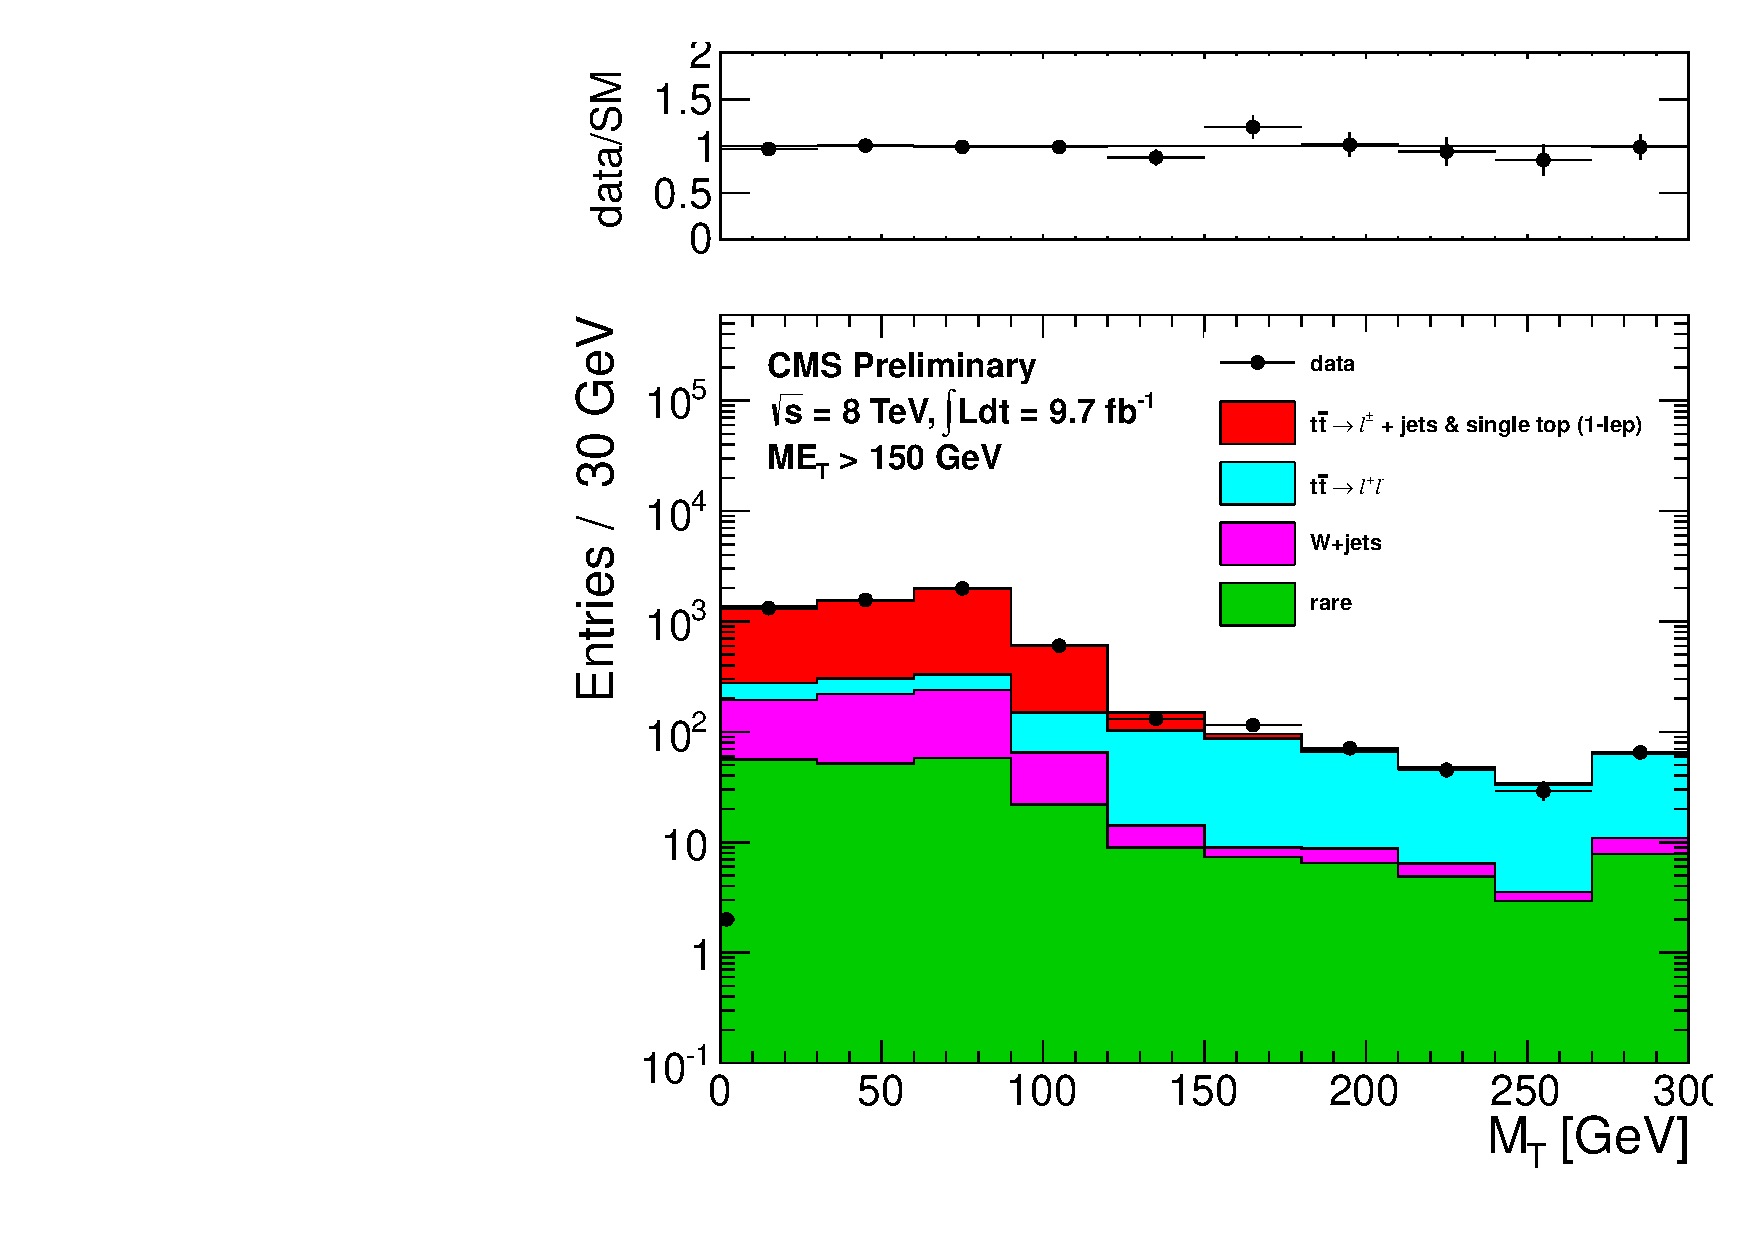
\includegraphics[width=0.5\linewidth]{plots/mt_met150_emucomb.pdf}
        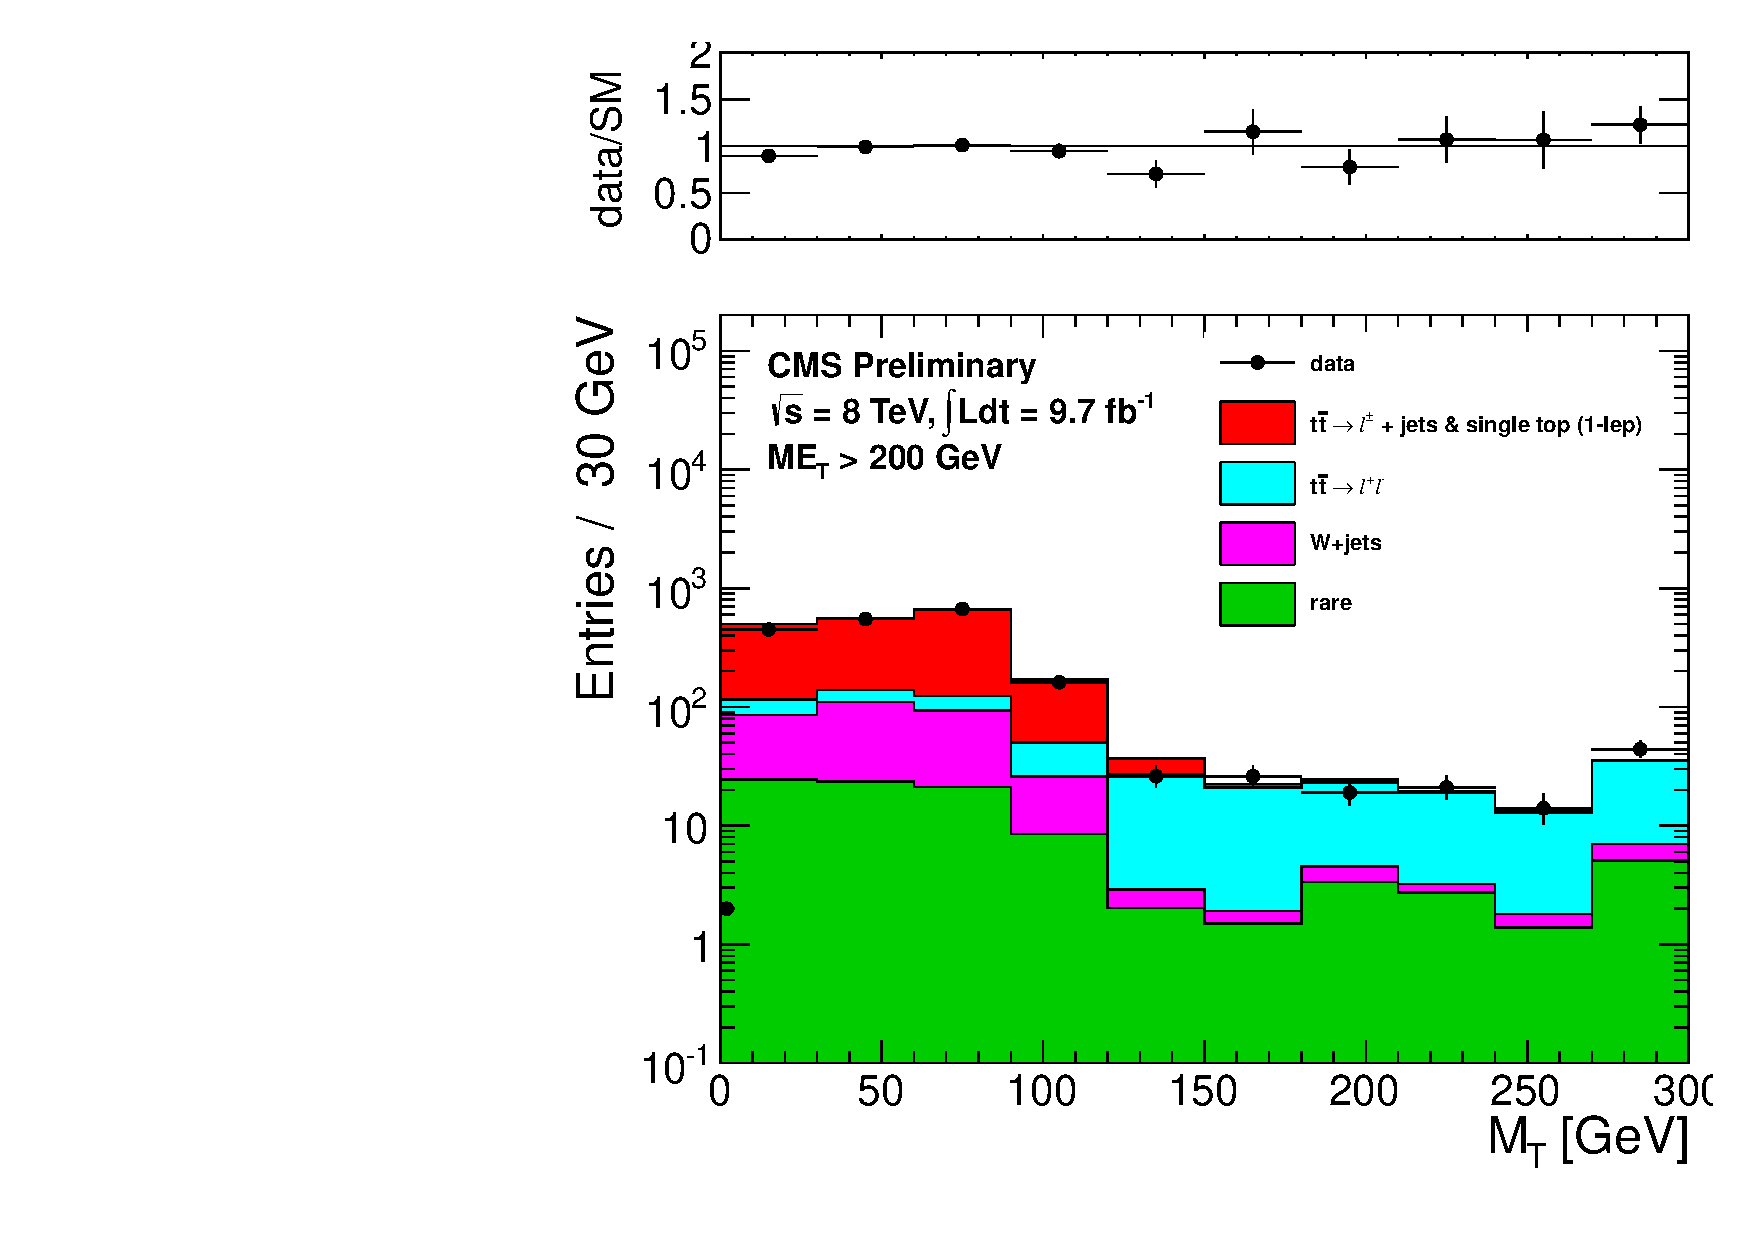
\includegraphics[width=0.5\linewidth]{plots/mt_met200_emucomb.pdf}%
        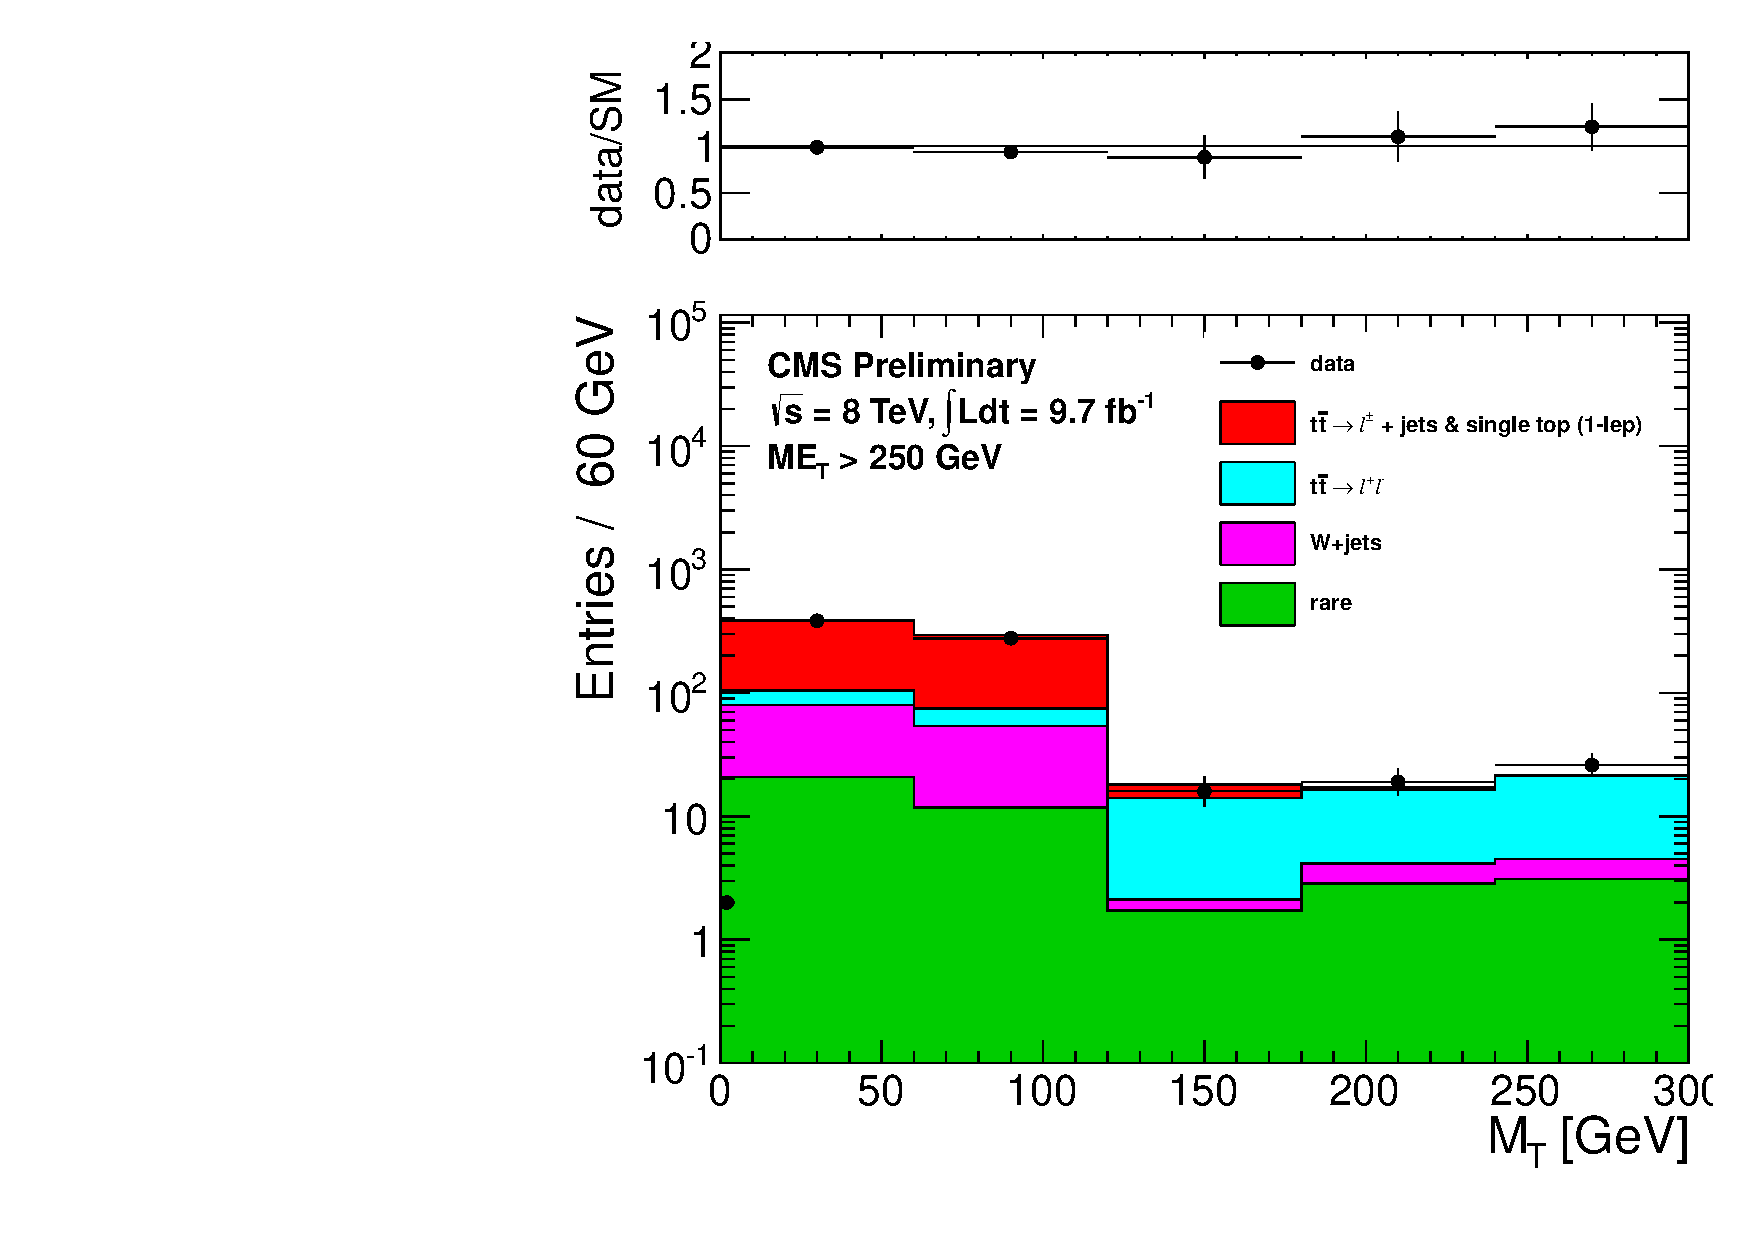
\includegraphics[width=0.5\linewidth]{plots/mt_met250_emucomb.pdf}
    \caption{$M_T$ in the data compared to SM Monte Carlo, for
      increasing values of \met. Only statistical uncertainties are
      shown. Note that the MC tails have not
      been rescaled at this point.
\label{fig:mtsig1}
}  
      \end{center}
\end{figure}

\begin{figure}[hbt]
  \begin{center}
        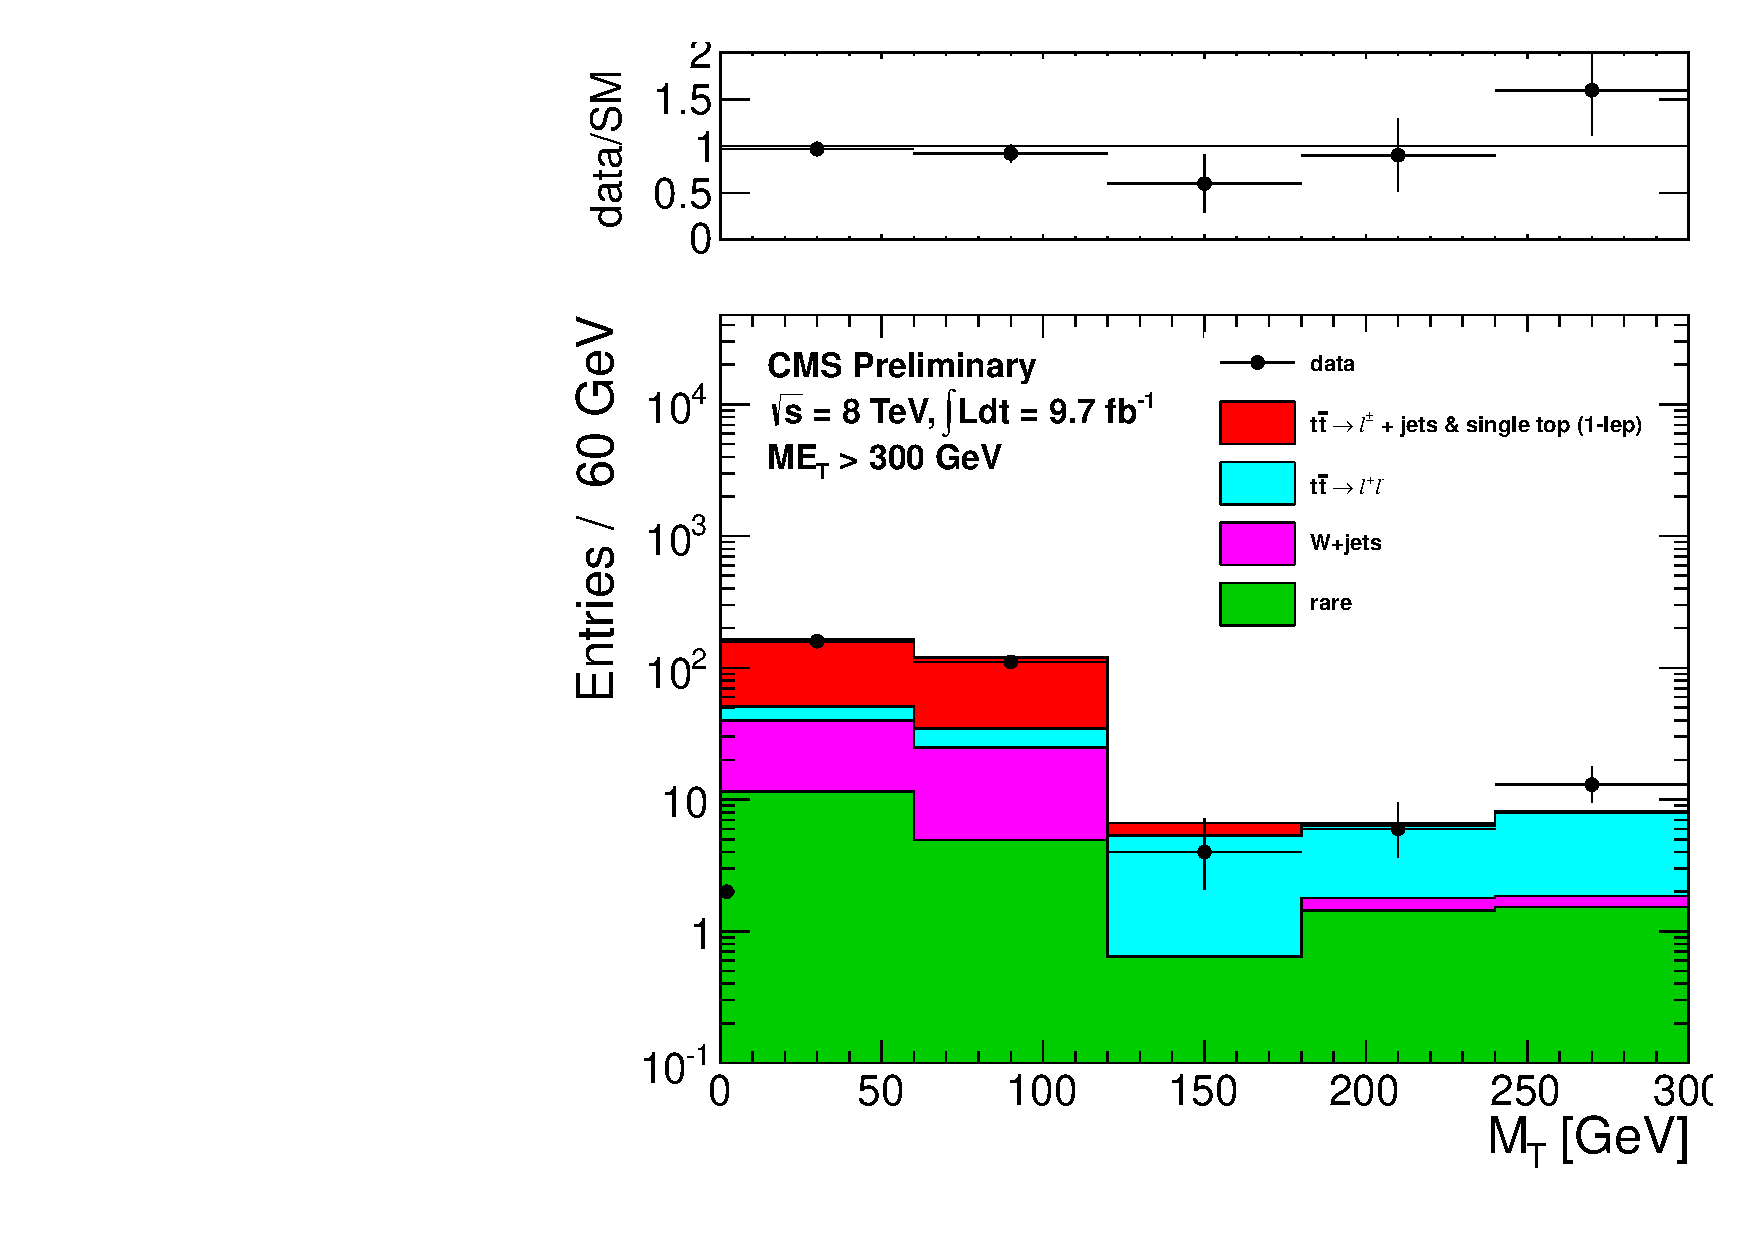
\includegraphics[width=0.5\linewidth]{plots/mt_met300_emucomb.pdf}%
        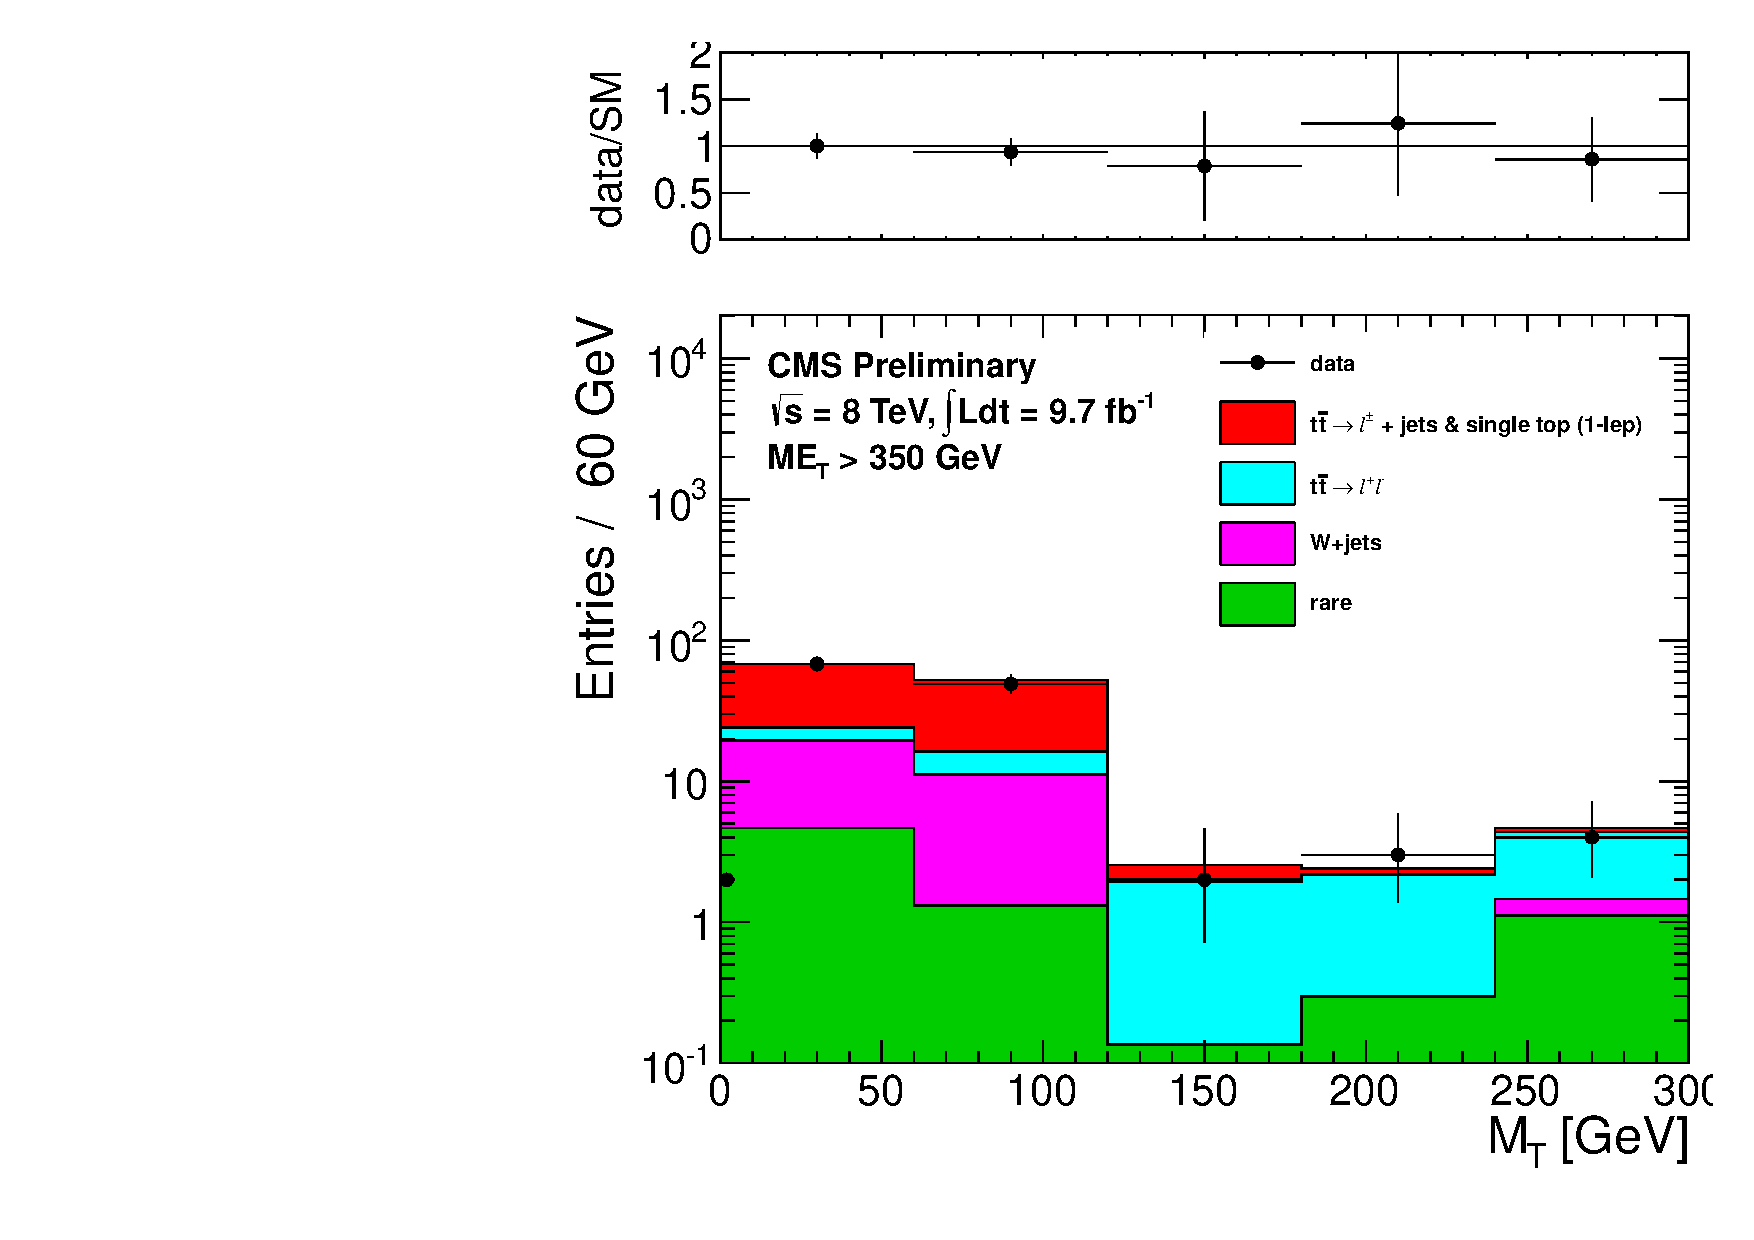
\includegraphics[width=0.5\linewidth]{plots/mt_met350_emucomb.pdf}
        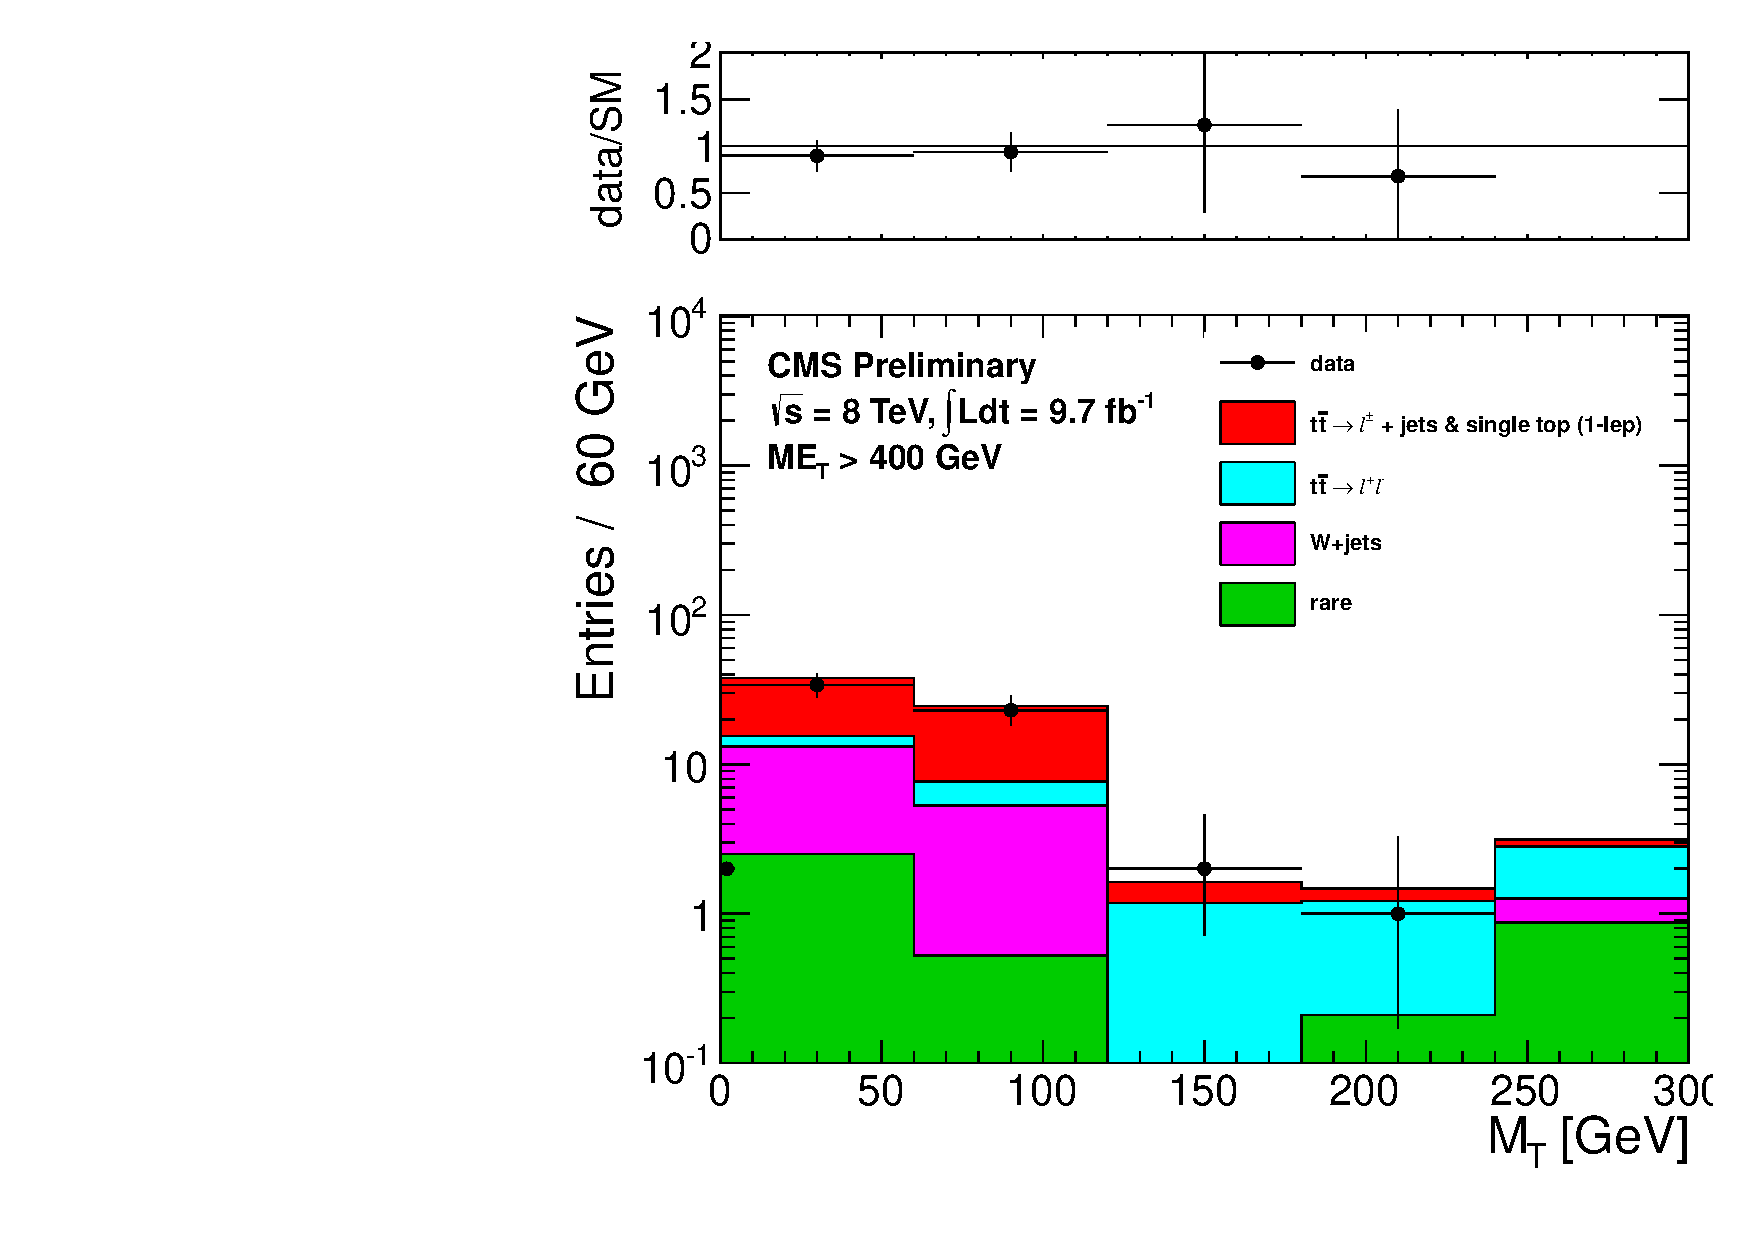
\includegraphics[width=0.5\linewidth]{plots/mt_met400_emucomb.pdf}
    \caption{$M_T$ in the data compared to SM Monte Carlo, for
      increasing values of \met. Only statistical uncertainties are
      shown. Note that the MC tails have not
      been rescaled at this point.
\label{fig:mtsig2}
}  
      \end{center}
\end{figure}


\clearpage
